\chapter{Marco Teórico}
\label{cap:marco_teorico}
En el presente capítulo se define con mayor detalle los conceptos revelantes que abarca esta tesis. El marco teórico incluye una breve descripción de lo que significa Aprendizaje colaborativo presentando además algunos de sus elementos y beneficios. Así mismo, también se describe algunas de las técnicas más conocidas para el aprendizaje colaborativo. Finalmente, se describe algunos conceptos sobre tecnologías para aplicaciones web, conceptos que serán de ayuda para la implementación de la presente tesis.
\section{Aprendizaje Colaborativo}
\subsection{Definición}
Existen diversas formas de definir lo que es Aprendizaje Colaborativo; \citeA{macgregor_collaborative_1990} dice que la enseñanza y el aprendizaje colaborativo son un enfoque educacional que involucra grupos de estudiantes trabajando juntos para resolver un problema, completar una tarea o crear un producto y \citeA{gerlach_1994} sostiene que el aprendizaje cooperativo está basado en la idea de que el aprendizaje es un acto social natural en el cual los participantes conversan entre sí mismos y que es a través de la comunicación y la charla donde realmente ocurre el aprendizaje.\\

El aprendizaje colaborativo es un término para describir una variedad de enfoques educacionales que implican reunir el esfuerzo intelectual de los estudiantes, o estudiantes y profesores juntos. Usualmente los estudiantes están trabajando en grupos de dos o más, buscando entender, solucionar problemas o crear productos. Las actividades de aprendizaje cooperativo son variadas, pero la mayoría se centran en la exploración del estudiante o la aplicación de los materiales de curso, no simplemente en la presentación de un tema por parte del profesor \cite{smith_collaborative_1992};además, el aprendizaje colaborativo tiene como principal característica una estructura que permite a lo estudiantes comunicarse entre sí, y es ahí donde ocurre el aprendizaje\cite{golub1988focus}.

\subsection{Elementos en el aprendizaje colaborativo}
\cite{johnson_1984} plantea 5 elementos básicos en el aprendizaje colaborativo. El aprendizaje colaborativo no es simplemente para los estudiantes el hecho de trabajar en grupo y de acuerdo con su investigación,  un ejercicio de aprendizaje sólo califica como colaborativo si están presentes los siguientes elementos:

\begin{itemize}
  \item \emph{La interdependencia positiva}. Los miembros del equipo están obligados a confiar en los demás para alcanzar un objetivo. Si uno de los miembros del equipo falla al realizar su parte, todos sufren las consecuencias. Los miembros del equipo necesitar creer que están unidos con los demás de una forma que aseguren el éxito en conjunto.
  \item \emph{La interacción ``cara a cara'' o simultánea}. Los miembros del equipo se tienen que ayudar y alentar entre sí para aprender. Ellos deben de explicar qué entendieron y así compartir su conocimiento.
  \item \emph{La responsabilidad individual}. Todos los estudiantes de un grupo son responsables de hacer su parte del trabajo.
  \item \emph{Habilidades sociales}. Los estudiantes deben ser alentados y ayudados a desarrollar y practicar la confianza de equipo, liderazgo, toma de decisiones, comunicación, y manejo de conflictos.
  \item \emph{Autoevaluación de grupo}. Los miembros del equipo tienen que fijarse objetivos, revisar periódicamente qué están haciendo bien como equipo, e identificar cambios por hacer con el fin de mejorar la efectividad a futuro.
\end{itemize}
\subsection{Beneficios del aprendizaje colaborativo}
Numerosos beneficios han sido descritos para el aprendizaje cooperativo \cite{panitz_1999}. Una buena forma de organizarlos es colocándolos en categorías. \citeA{johnsons_1989, panitz_1999} hicieron una lista de más de 50 beneficios para el aprendizaje cooperativo, algunos de los cuales se presentan a continuación:

\begin{enumerate}
  \item Beneficios sociales
  \begin{enumerate}
    \item Ayuda a desarrollar un sistema de apoyo social para los estudiantes.
    \item Lleva a construir un entendimiento de la diversidad entre los estudiantes y el personal.
    \item Establece un entorno positivo para modelar y practicar la cooperación y el trabajo en equipo.
    \item Desarrolla comunidades de aprendizaje.
  \end{enumerate}
  \item Beneficios psicológicos
  \begin{enumerate}
    \item La instrucción centrada en los estudiantes aumenta la autoestima de los mismos.
    \item La cooperación reduce la ansiedad.
    \item El aprendizaje cooperativo desarrolla actitudes positivas hacia los profesores.
  \end{enumerate}
  \item Beneficios académicos
  \begin{enumerate}
    \item El aprendizaje cooperativo promueve habilidades de pensamiento crítico.
    \item Envuelve a los estudiantes activamente en el proceso de aprendizaje.
    \item Los resultados de clase son mejorados.
    \item El aprendizaje cooperativo modela técnicas apropiadas para la resolución de problemas.
    \item Grandes conferencias pueden ser personalizadas.
    \item El aprendizaje es especialmente útil para motivar a los estudiantes en un plan de estudios específico.
  \end{enumerate}
\end{enumerate}

\section{Técnicas de Aprendizaje Colaborativo}

\subsection{La técnica de Jigsaw}

La técnica de Jigsaw, que fue introducida por \citeA{aronson_jigsaw_1978} para mejorar la cooperación en pares y crear solidaridad en equipo entre los estudiantes a través de la división de tareas, involucra a cada estudiantes en un grupo a asumir responsabilidades en el aprendizaje. En consecuencia, los estudiantes trabajan en dos diferentes grupos: el grupo de expertos y el grupo jigsaw.\\

Los objetivos de está técnica son:

\begin{itemize}
  \item Estructurar las interacciones entre los alumnos, mediante equipos de trabajo.
  \item Lograr que los alumnos dependan unos de otros para lograr sus objetivos.
\end{itemize}

La secuencia de pasos que conforman esta técnica son los siguientes \footnote{\cite{upm_2008}}:

\begin{enumerate}
  \item El docente debe tener preparada la división del tema a tratar en cinco o séis documentos, los cuales se repartirán a los alumnos siguiendo un orden. Cada uno de ellos será necesario para aprender la totalidad del tema, y por lo tanto, todos ellos formarán la unidad temática completa.
  \item Se divide a los alumnos en grupos de cinco o séis(según el número de documentos elaborados) y dentro de cada grupo cada miembro recibirá un número de 1 a 5(ó 6). Ver figura \ref{fig:jigsaw01}

\begin{figure}[h]
  \centering
  % Requires \usepackage{graphicx}
  \fbox{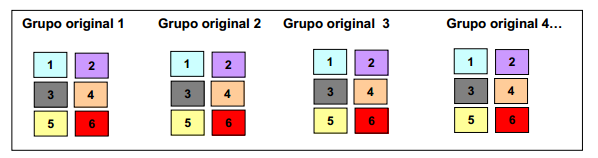
\includegraphics[scale=0.6]{figuras/jigsaw01.png}}\\
  \caption{Grupos originales en la técnica Jigsaw}\label{fig:jigsaw01}
\end{figure}

A los estudiantes con el número 1 se les reparte el mismo documento, que será diferente al resto de los compañeros y que puede corresponderse a la primera parte del tema de estudio. A los alumnos con el número 2 se les reparte otro documento y así sucesivamente.

La primera fase será, por tanto, que los alumnos preparen su documento de forma individual, que lo lean, que lo entienda, que lo aprendan y que recopilen las dudas que surjan.

  \item Una vez que ya ha finalizado el tiempo estimado para la preparación individual del documento, comienta la segunda fase que se denomina ``Reunión de expertos''. En este momento todos los alumnos con el mismo número se reúnen para debatir y comentar sobre el documento que les fue asignado. Ver figura \ref{fig:jigsaw02}

  \begin{figure}[h]
  \centering
  % Requires \usepackage{graphicx}
  \fbox{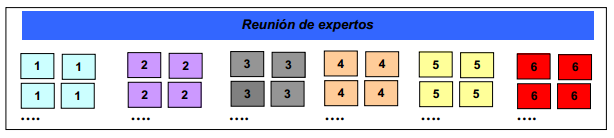
\includegraphics[scale=0.6]{figuras/jigsaw02.png}}\\
  \caption{Grupos de expertos}\label{fig:jigsaw02}
\end{figure}

    \item Finalizada las reuniones de expertos, llega la tercera fase, que supone el regreso al grupo original y, cada alumno explicará al resto de sus compañeros el documentos que ha estado preparando. Ver figura \ref{fig:jigsaw03}

\begin{figure}[h]
  \centering
  % Requires \usepackage{graphicx}
  \fbox{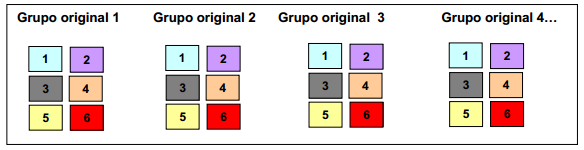
\includegraphics[scale=0.6]{figuras/jigsaw03.png}}\\
  \caption{Regreso a los originales}\label{fig:jigsaw03}
\end{figure}

\item La última fase, consiste en evaluar el aprendizaje logrado y la eficacia de la técnica individualmente. Para ello, el docente prepara un test sobre todo el material que ha sido trabajado durante la sesión de clase.

\end{enumerate}

\subsection{Programación en pares}
Una técnica educacional que tiene elementos en común con el aprendizaje cooperativo es la programación en pares. En esta forma de colaboración, dos programadores trabajan lado a lado en un computador. En cualquier momento, un miembro del equipo(``the driver'') está escribiendo en el computador o transcribiendo algún diseño elaborado. El otro integrante del equipo (``the navigator'') está observando activamente el trabajo del primero, buscando defectos, pensando en otras alternativas de solución, haciendo preguntas, etc. Los roles de ``driver'' y ``navigator'' son intercambiados periódicamente entre ambos miembros del equipo.\\

La programación en pares fue originalmente popularizada como parte de la metodología de desarrollo de software XP \cite{beck_extreme_2000}. Así mismo, resultados de investigaciones muestran que los programadores en pares producen código de mayor calidad en mitad de tiempo que lo programadores individuales \cite{williams2000collaborative,williams_strengthening_2000}. La técnica de programación en pares también has mostrado ser efectiva para estudiantes de programación, logrando mejorar el aprendizaje en los alumnos\cite{mcdowell_effects_2002}.

%\subsection{El estudio de Casos}
%Es una técnica de aprendizaje cooperativo, la cual está basada en un enfoque de estudio de problemas. \cite{JCAL:JCAL119}. Durante un Estudio de Casos, los estudiantes reciben materiales que describen una situación en concreto y se les pide analizarla tratando de identificar los puntos fuertes y débiles del caso, así como también se les pide reflexionar sobre posibles soluciones que pudiesen añadir a las ya presentadas en el problema. El factor más importante del Estudio de Casos es que éstos están basados en problemas y/o situaciones reales \cite{JCAL:JCAL119}.
%

\section{Tecnologías web}


\subsection{AJAX}

El término AJAX es un acrónimo de Asynchronous JavaScript $+$ XML que puede traducirse como ``JavaScript asíncrono más XML''. El término AJAX se presentó por primera vez en el artículo ``Ajax, A new Approach to Web Applications" publicado por Jesse James Garret en el año 2005. En realidad, en dicho artículo se dice que AJAX no es una tecnología en sí mismo sino un conjunto de varias tecnologías que se unen de formas nuevas y sorprendentes \cite{ajax_dummies_2006}.\\

AJAX está compuesto por los siguiente:

\begin{itemize}
  \item La presentación en el navegador está basada en HTML y CSS.
  \item Document Object Model (DOM), para la interacción y manipulación dinámica de la presentación.
  \item XML, XSLT y JSON, para el intercambio y la manipulación de información
  \item XMLHttpRequest, para el intercambio asíncrono de información.
  \item JavaScript, para unir todas las tecnologías antes mencionadas.
\end{itemize}
%Ver figura \ref{fig:ajax}
\begin{figure}[h]
  \centering
  % Requires \usepackage{graphicx}
  \fbox{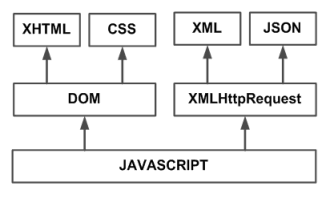
\includegraphics[scale=0.8]{figuras/ajax_01.png}}\\
  \caption{Tecnologías agrupadas bajo el concepto de AJAX}\label{fig:ajax}
\end{figure}

JavaScript es un lenguaje que la mayoría de navegadores soporta y que permite manipular datos entre la vista y el servidor. A continuación se indica cómo es que AJAX funciona:\cite{ajax_dummies_2006}

\begin{enumerate}
  \item En el navegador se escribe código en JavaScript con el cual se puede obtener información del servidor las veces que sean necesarias.
  \item Cuando más data es requerida, el JavaScript usa el objeto XMLHttpRequest para enviar la petición al servidor sin necesidad de refrescar toda la página web.
  \item La data que retorna desde el servidor puede estar en formato XML o puede ser sólo texto plano. Lo importante es que el JavaScript en el navegador puede leer la información recibida y mostrarla en la vista.
\end{enumerate}

\subsubsection{¿Qué se puede hacer con AJAX?}

AJAX ha estado presente desde 1998 y muchas aplicaciones como Microsoft's Outlook Web Access la han usado. Sin embargo, recien a partir del año 2005 cuando AJAX tomó sitio en el campo del desarrollo web después de que fuese utilizado en aplicaciones como Google Suggest y Google Maps.\cite{ajax_dummies_2006}\\

Desde entonces, AJAX ha permitido realizar diferentes tipos de aplicaciones web como por ejemplo:

\begin{itemize}
  \item \emph{Búsqueda en tiempo real}. Una de las mejores cosas que se puede realizar usando AJAX son las búsquedas en vivo, donde el usuario obtiene lo que busca mientras va escribiendo lo que necesita buscar.
  \item \emph{Obtener la respuesta con autocompletado}. Muy parecido a las búsquedas en vivo son las aplicaciones que tratan de adivinar la palabra que estamos escribiendo obteniendo una lista de palabras similares del servidor que son puestas a nuetra vista.
  \item \emph{Chatear con amigos}. Puesto que AJAX no necesita refrescar toda la página web, es una buena herramienta para realizar programas de chat donde muchos usuarios conversan al mismo tiempo.
  \item \emph{Dragging and Dropping}.
  \item \emph{Juegos con AJAX}.
  \item \emph{Menús pop up}. Se puede obtener data desde el servidor tan pronto como sea necesario usando Ajax.
\end{itemize}

\subsection{Polling}
Después del posicionamiento de AJAX, no pasó mucho tiempo para tratar de lograr que los eventos en el navegador salieran fuera de la ecuación y se pudiera automatizar el proceso de obtener nueva información desde el servidor. Fue entonces que los desarrolladores establecieron un intervalo de actualización para revisar actualizaciones cada $n$ segundos \cite{lengstorf_realtime_2013}. Ver figura \ref{fig:polling}

\begin{figure}[!h]
  \centering
  % Requires \usepackage{graphicx}
  \fbox{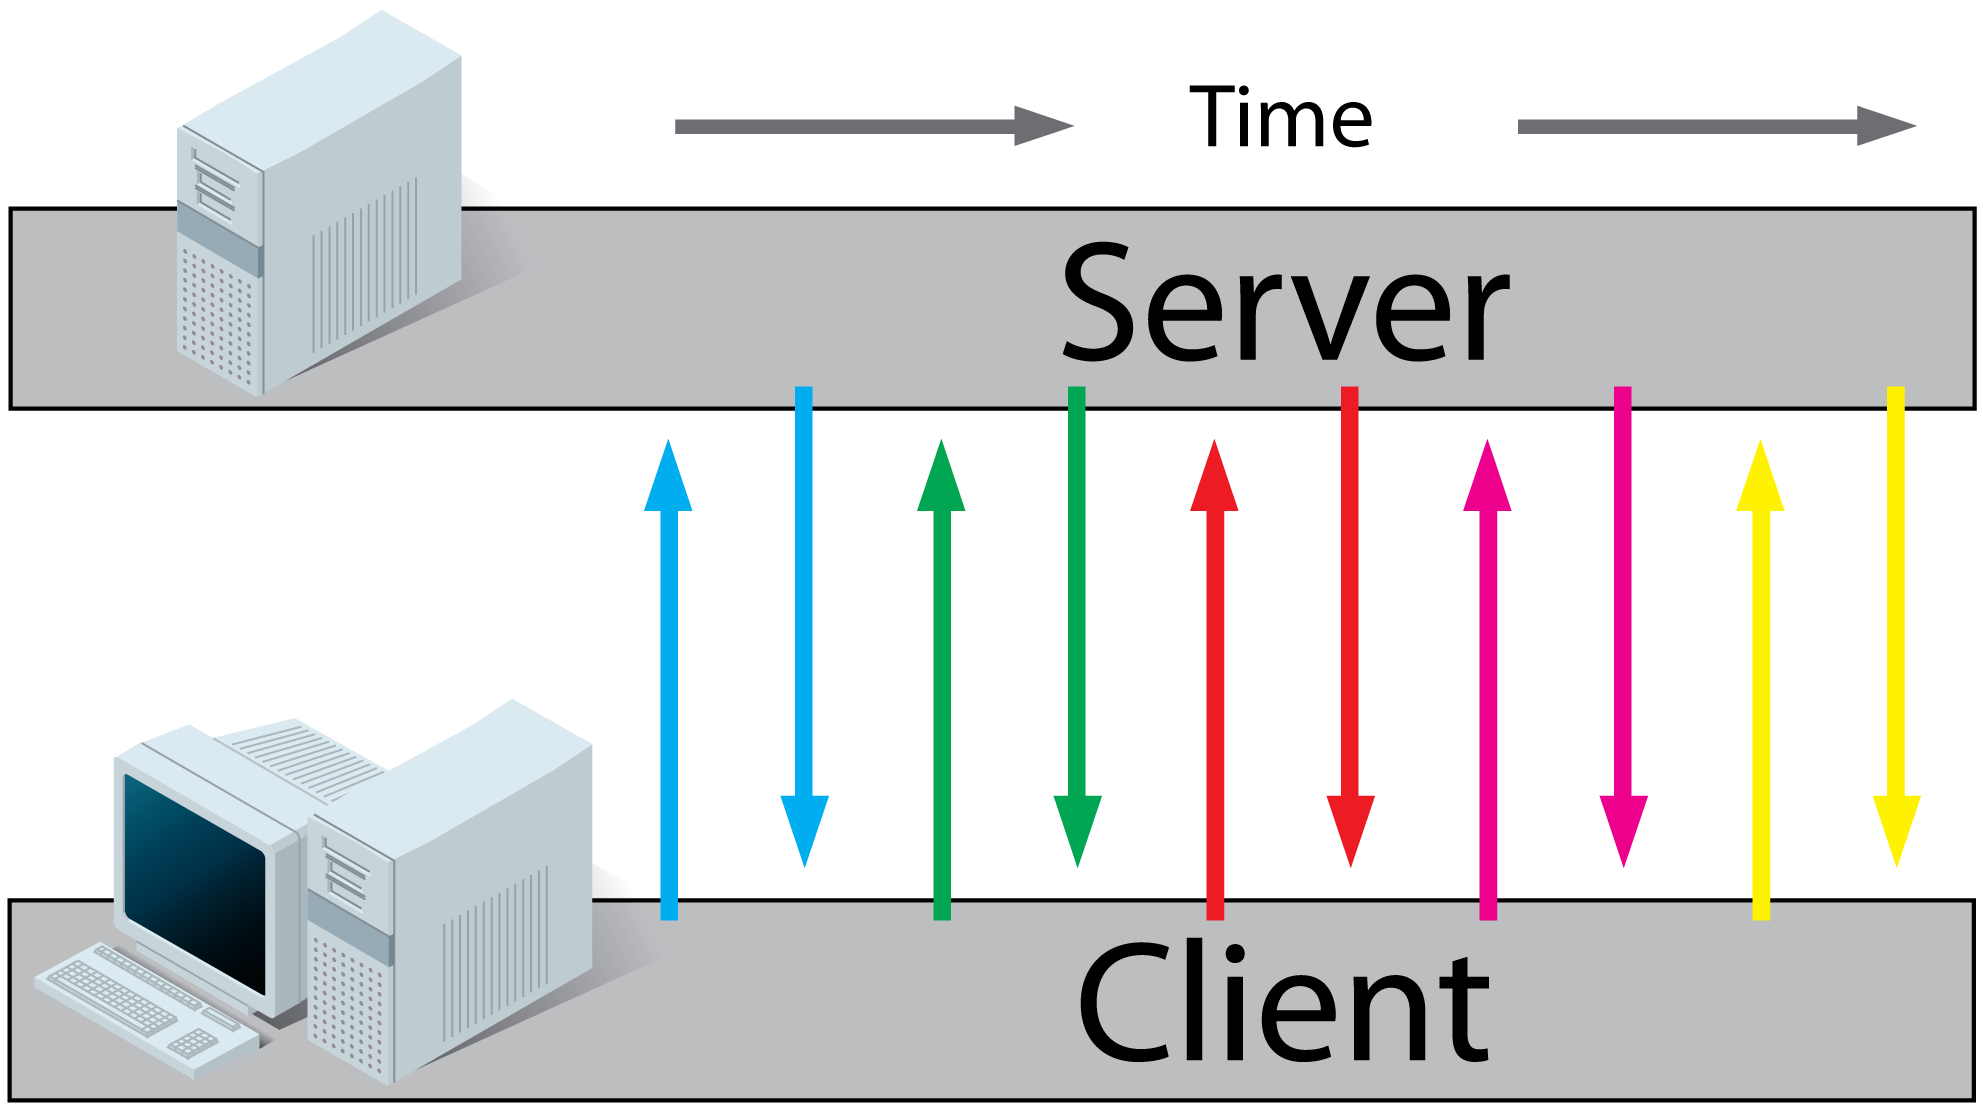
\includegraphics[scale=0.6]{figuras/ajax_polling.png}}\\
  \caption{Polling}{A través del Polling se envía peticiones HTTP para comprobar si existe nueva información.}\label{fig:polling}
\end{figure}

\subsection{HTTP Long-Polling}
El siguiente paso en la evolución del tiempo real es el HTTP \emph{long-polling}, el cual consiste en abrir una petición HTTP por un periodo de tiempo para escuchar respuestas del servidor. Si hubiese nueva data, el servidor la enviaría y se cerraría la petición; de otro modo, la petición es cerrada después de un intervalo de tiempo límite y se abre una nueva petición \cite{lengstorf_realtime_2013}.  Ver figura \ref{fig:http_long_polling}
\begin{figure}[h]
  \centering
  % Requires \usepackage{graphicx}
  \fbox{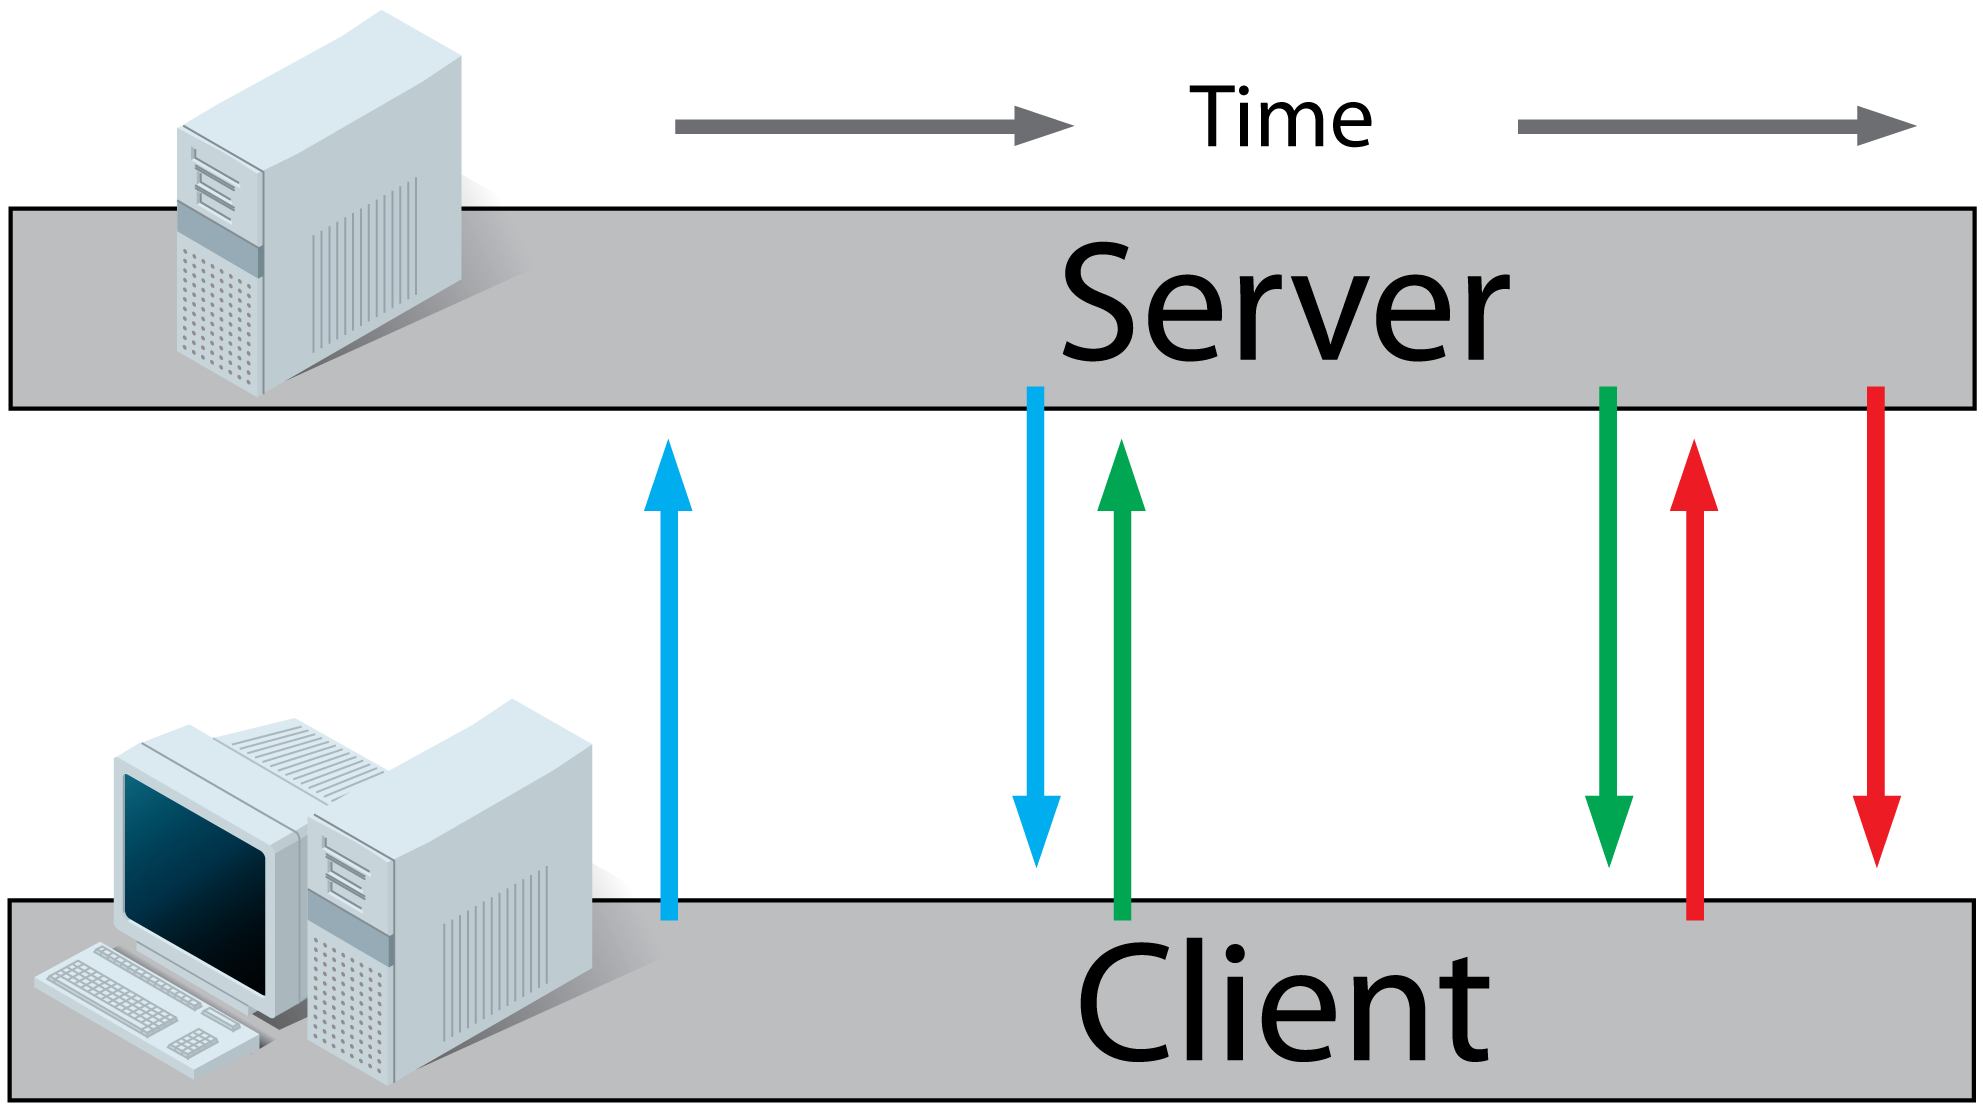
\includegraphics[scale=0.6]{figuras/ajax_long_polling.png}}\\
  \caption{Long Polling}{Gracias al HTTP Long-polling, se mantiene abierta una peticion HTTP por un periodo de tiempo para comprobar si existe nueva información.}\label{fig:http_long_polling}
\end{figure}
%%\cite{lengstorf2013realtime}

\subsection{WebSockets}
Web sockets (Ver figura \ref{fig:websockets}) es una tecnología que proporciona un canal de comunicación bidireccional y full-duplex sobre una única conexión TCP en los navegadores y servidores web. A comparación de HTTP, WebSocket puede reducir efectivamente el tráfico de red innecesario, a través de una forma estandarizada para que el servidor envíe contenido al navegador sin que éste sea solicitado.\cite{cheng_new_2013}\\

\begin{figure}[h]
  \centering
  % Requires \usepackage{graphicx}
  \fbox{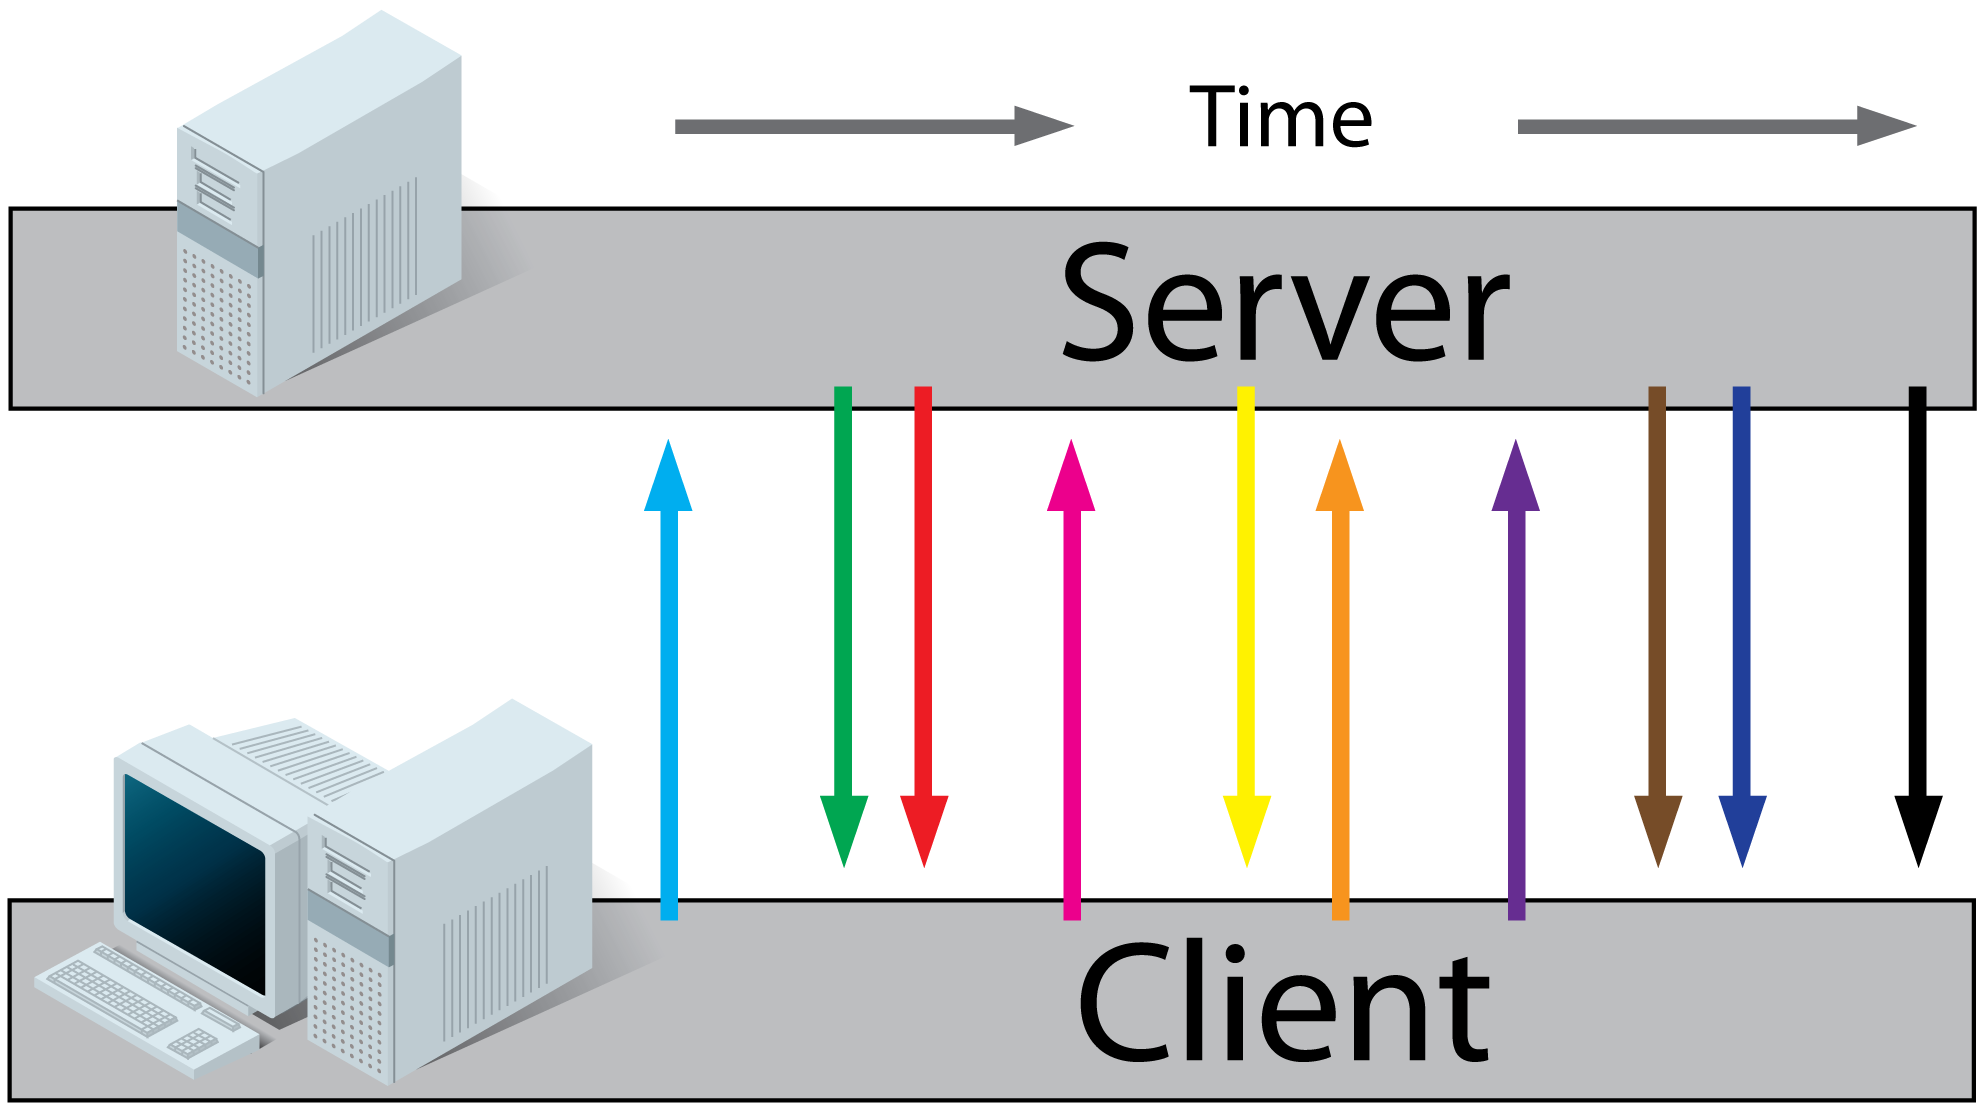
\includegraphics[scale=0.6]{figuras/websockets.png}}\\
  \caption{Websockets}{Una nueva tecnología para la comunicación bidireccional.}\label{fig:websockets}
\end{figure}

\subsubsection{¿Por qué usar Websockets?}

Existen muchas razones que no conllevan a utilizar websockets cuando desarrollemos una aplicación web. Algunas de ellas se mencionan a continuación:

\begin{itemize}
  \item Websockets permite que la comunicación en tiempo real sea mucho más eficiente. Desde luego, siempre será posible usar polling sobre HTTP para recibir las notificaciones desde el servidor. Sin embargo, con el uso de Websockets se ahorra ancho de banda, cpu, y latencia.
  \item La comunicación entre el cliente y el servidor se vuelve más sencilla.
\end{itemize}

Los websockets tiene una gran acogida de parte de la comunidad de desarrolladores, lo cual se ve reflejado en la variedad de implementaciones de websockets como Apache mod\_pywebsocket, Jetty, Socket.IO, entre otros.


\section{Glosario}

\begin{enumerate}
  \item \textbf{Framework}. La palabra inglesa "framework" (marco de trabajo) define, en términos generales, un conjunto estandarizado de conceptos, prácticas y criterios para enfocar un tipo de problemática particular que sirve como referencia, para enfrentar y resolver nuevos problemas de índole similar.
  \item \textbf{Librería}. En informática, una librería es un conjunto de implementaciones funcionales, codificadas en un lenguaje de programación, que ofrece una interfaz bien definida para la funcionalidad que se invoca.
  \item \textbf{Socket}. Designa un concepto abstracto por el cual dos programas (posiblemente situados en computadoras distintas) pueden intercambiar cualquier flujo de datos, generalmente de manera fiable y ordenada.
%  \item \textbf{Tiempo real}. Un sistema en tiempo real (STR) es aquel sistema digital que interactúa activamente con un entorno con dinámica conocida en relación con sus entradas, salidas y restricciones temporales, para darle un correcto funcionamiento de acuerdo con los conceptos de predictibilidad, estabilidad, controlabilidad y alcanzabilidad
  \item \textbf{CSCL}. Computer-Supported Collaborative Learning. Aprendizaje colaborativo apoyado por computador.
  \item \textbf{API}. Application Programming Interface. Es el conjunto de funciones y procedimientos que ofrece cierta librería para ser utilizado por otro software como un capa de abstracción. Representa la capacidad de comunicación entre componentes de un software.
\end{enumerate}













